\documentclass[10pt]{article}
\usepackage[margin=.65in]{geometry}
\usepackage{graphicx,booktabs,hyperref,amsmath,amssymb,array}
\hypersetup{colorlinks=true,urlcolor=blue}
\setlength{\parindent}{0pt}
\setlength{\parskip}{5pt}
\newcommand{\Frob}{\operatorname{Frob}}
\newcommand{\Eminus}{E(K)^{-}}
\begin{document}
\begin{center}
{\Large The explicit twist map is a group isomorphism}\\[4pt]
{\large Onto the entire Frobenius-minus eigenspace}\\[4pt]
23 October 2026 $\cdot$ \texttt{group-map-20261023} $\cdot$ PR \#2381
\end{center}
\textbf{Checked result.} Lean proves addition and integer-scalar compatibility
of the existing actual-point quadratic-twist map, transports source annihilators,
and identifies its entire minus eigenspace. Rational base-change points give
exactly the fixed eigenspace. The unmodified repository proof gate passes
\textbf{49 named research theorems / 57 audited declarations}, zero failing
and zero extra trusted axioms. This closes a formal bridge; it is not a solver
speedup, a hardness proof, or a universal no-connection theorem.

Let $k$ be finite of odd characteristic, $q=\#k$, $d$ a nonsquare, $K/k$ any
field algebra containing $u^2=d$, and $E:y^2=x^3+ax+b$ elliptic. Set
\[
E_d:Y^2=X^3+d^2aX+d^3b,\qquad
\psi(O)=O,\quad\psi(X,Y)=\left(X/d,Y/(du)\right).
\]
There is no hidden finite-extension or degree-two hypothesis on $K$.
The earlier proof derived $u^q=-u$ and actual Frobenius negation; its source
and all old certificates remain unchanged.

\begin{center}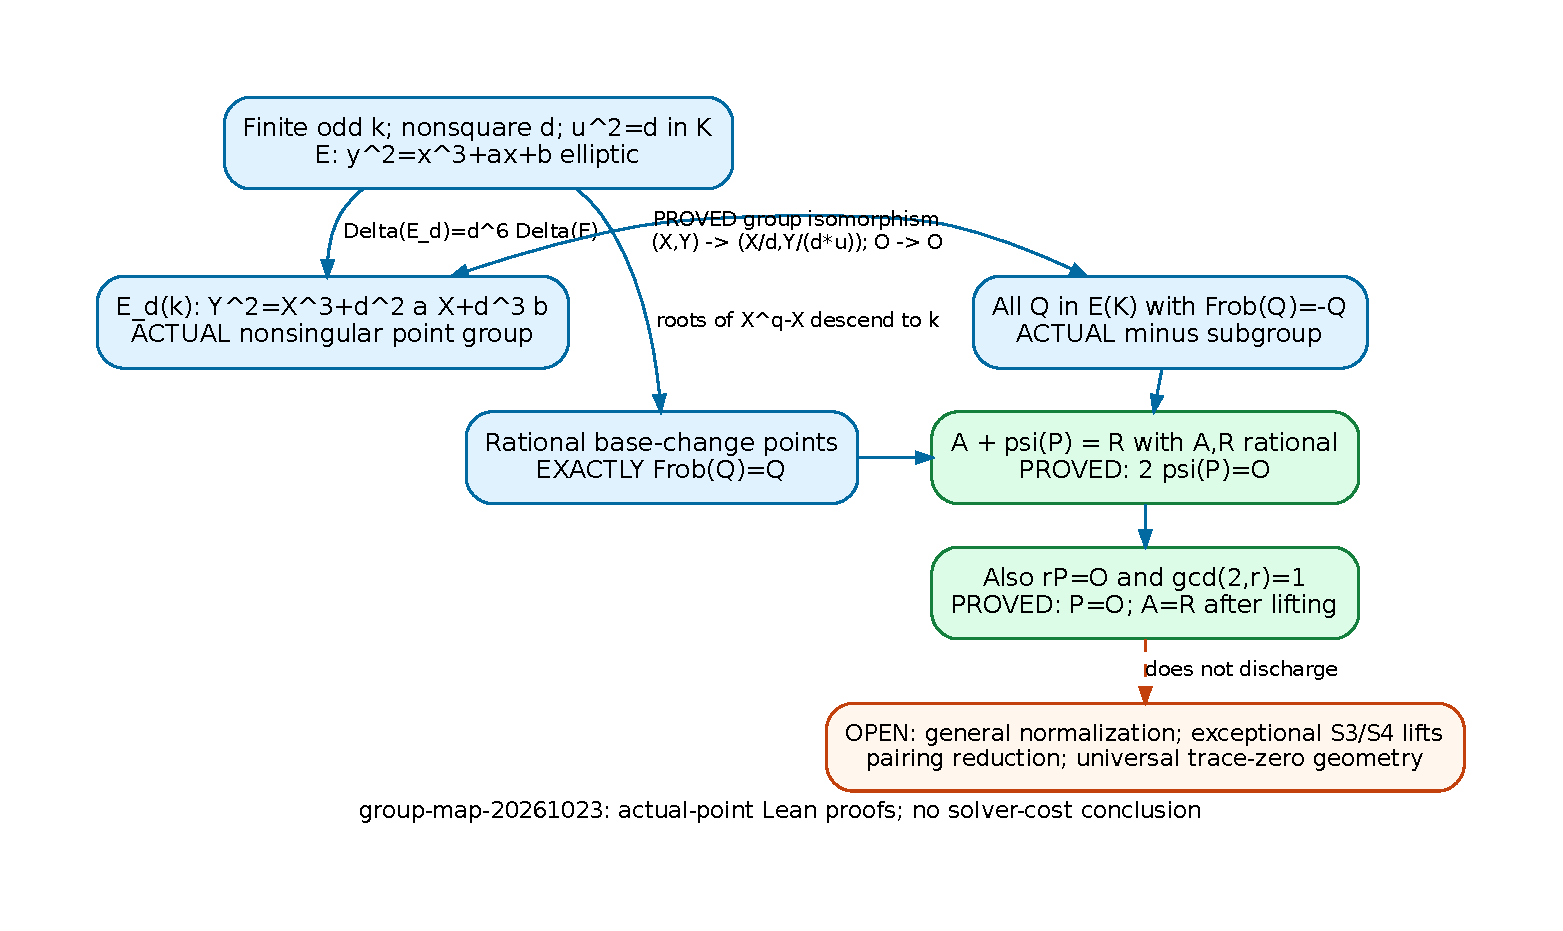
\includegraphics[height=4.05in,width=\linewidth,keepaspectratio]{bridge.pdf}\end{center}

\textbf{Source-order obstruction.} For rational lifts $A,R$, if
$A+\psi(P)=R$, $rP=O$ and $\gcd(2,r)=1$, then $P=O$ and the rational lifts
are equal. The annihilator now comes from the source point through the
proved group map. For a finite sum, only the aggregate is forced to zero;
individual summands need not vanish. Nonzero two-torsion remains an exception
when oddness is dropped.

\newpage
\begin{center}{\Large What the checked proof actually does}\end{center}
\textbf{Addition.} The new \texttt{TwistGroupMap} module proves that the
secant, tangent and vertical slopes transform by $1/u$. Addition's x and y
coordinates transform by $1/d$ and $1/(du)$. The proof on Mathlib's actual
nonsingular points includes $O$, inverse pairs and doubling; it does not
assume compatibility. It constructs an actual additive homomorphism, proves
\[
\psi(P+Q)=\psi(P)+\psi(Q),\quad
\psi([n]P)=[n]\psi(P)\ (n\in\mathbb Z),\quad
[r]\psi(P)=O\ \Longleftrightarrow\ [r]P=O.
\]
The group-map part needs fields, $d\ne0$, $u^2=d$ and the elliptic short model.
Finiteness, odd characteristic and nonsquareness enter the Frobenius consequences.

\textbf{Full minus eigenspace.} The new \texttt{TwistEigenspace} module first
proves $z^q=z$ iff $z$ comes from $k$, using all roots of $X^q-X$ and the
injective algebra map. The fixed field is derived, not assumed. If
$Q=(x,y)$ satisfies $\Frob(Q)=-Q$, then $\Frob(x)=x$ and $\Frob(y)=-y$.
Since $\Frob(u)=-u$, both $dx$ and $duy$ are fixed. They therefore descend
to $X,Y\in k$. Substitution proves the actual equation of $E_d$, and
\[
\Delta(E_d)=d^6\Delta(E)\ne0
\]
gives nonsingularity. The reconstructed source point maps to $Q$.
This includes infinity and two-torsion. Combined with the proved addition
and injection, \texttt{liftEquivMinus} is a genuine group isomorphism
\[
E_d(k)\ \simeq\ \{Q\in E(K):\Frob(Q)=-Q\}.
\]
The same fixed-field argument descends both coordinates of every fixed
actual point on an elliptic Weierstrass model, proving exactly the rational
plus-space description. This does not say every point is in either subgroup
or assert a direct-sum decomposition at two-torsion.

\textbf{Proof map.} The canonical \path{lean/README.md} maps every claim to
its declaration and exact hypotheses. The new modules contribute 21 named
theorems: 16 group/coordinate statements and five fixed-field, discriminant
and eigenspace statements. The gate also checks eight older generated helpers.
Only \texttt{propext}, \texttt{Classical.choice} and \texttt{Quot.sound} occur;
there are no added research axioms, placeholders, or trusted native evaluations.
\texttt{lean4checker --fresh} is unavailable; no extra external replay is claimed.

\textbf{Pinned sources and evidence.} Lean 4.34.1 and Mathlib
\texttt{d13f23b723b8a846827a245b89c10fc7d3f11612} remain pinned.
Protocol commit \texttt{6fb418e8a} preceded execution. The exact new sources,
all failed attempts and the passing build/axiom receipts are retained in
\path{validation/group-map-20261023/}. Provisional axiom printouts from a
failed elaboration are not proof receipts. The actual passing gate covers
all five modules.

\newpage
\begin{center}{\Large Native controls and the PR-caused catalog repair}\end{center}
Four native IDC1 certificates bind the exact new Lean sources. Each replays
32 derived points and 16 extra points. Each false plus-one identity is rejected
arithmetically with a saved counterexample, and each false source hash is rejected.
The records cover polynomial parts; Lean separately checks inverses, points,
addition and Frobenius.

\begin{center}\small
\begin{tabular}{ll}
\toprule
Polynomial part & Certificate id\\\midrule
Tangent numerator & \texttt{IDC1h501f62832dc059fb}\\
Addition x coordinate & \texttt{IDC1he0c463dc2e585208}\\
Addition y coordinate & \texttt{IDC1hfb09521ce1a737cb}\\
Discriminant scaling & \texttt{IDC1hb3a3c677428bc4b1}\\\bottomrule
\end{tabular}\normalsize\end{center}

\textbf{Metadata defect reproduced.} The registry gained 1,921 models in
this PR, but the Jacobian-transfer report still covered 2,572. The unchanged
native generator accepts the old base registry and rejects the old report
with the new registry. Under separately committed protocol \texttt{ea1929fd9},
the catalog is regenerated at its unchanged 200,000 factor budget.

\begin{center}\small
\begin{tabular}{lrr}
\toprule
Catalog field & Before & After\\\midrule
Models & 2,572 & 4,493\\
Declared formula routes & 6,565 & 11,365\\
Boundary verdicts & 1,917 & 3,838\\
Formula advantage / marginal & 598 / 57 & 598 / 57\\\bottomrule
\end{tabular}\normalsize\end{center}
Every prior per-model object and the cost model remain equal; exact registry
membership has no missing or duplicate model. The registry itself is unchanged.
Native checks, table/query/chart commands and altered-file rejection pass.
The marked Markdown summary table is byte-identical after regeneration.
The strict cover assessment's source binding and inventory-freshness statement
are refreshed; all other assessment sections and transfer verdicts remain equal.

\begin{center}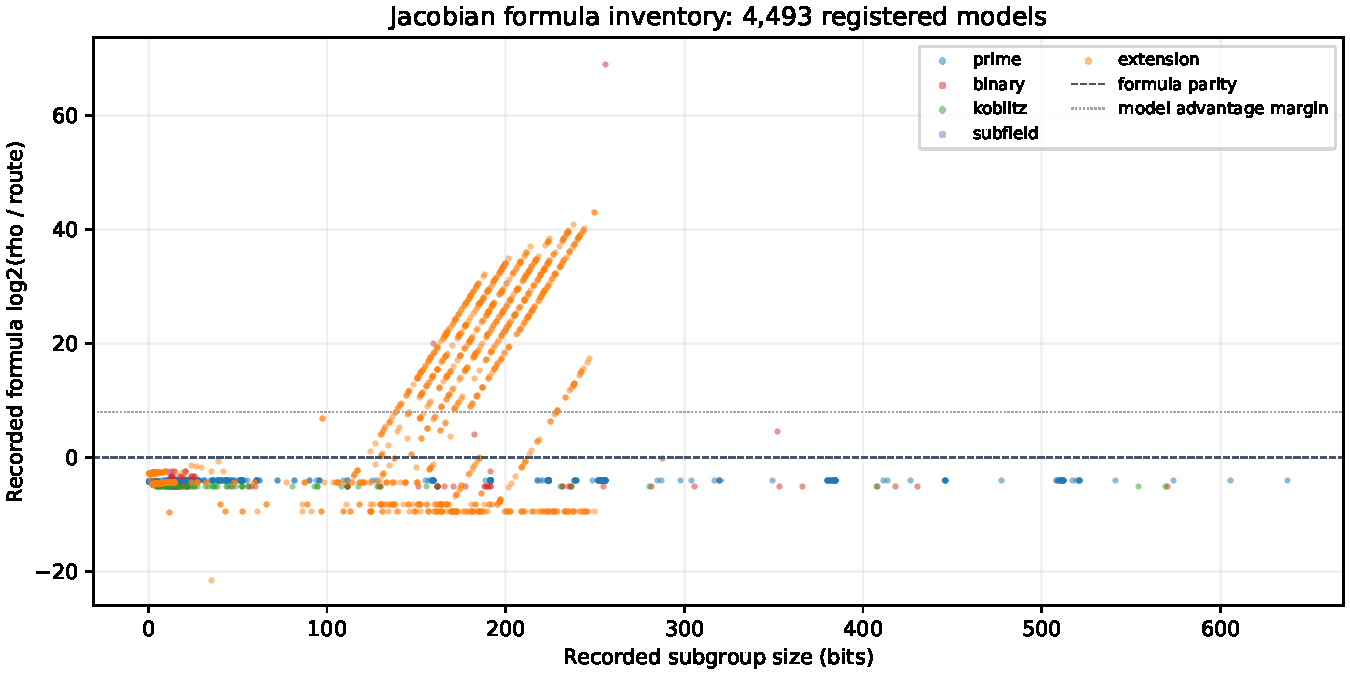
\includegraphics[width=.95\linewidth]{jacobian-readable.pdf}\end{center}
\small Recorded native values, \texttt{jacobian-transfers/2}, all 4,493 models.
Axes are subgroup bits and formula $\log_2(\rho)-\log_2(\mathrm{route})$.
Points are conditional formula leads, not constructed transfers, timings,
speedups or security claims. Plotting performs layout only; raw native SVG/TikZ
are retained. No sampling uncertainty is asserted.\normalsize

\newpage
\begin{center}{\Large Validation, limits and next discriminating step}\end{center}
\begin{tabular}{p{.39\linewidth}p{.56\linewidth}}
\toprule
Requirement & Actual outcome\\\midrule
Study proof gate & PASS: 57 declarations, zero failing/trusted\\
New native certificates & Four exact-byte replays; false identities and source hashes rejected\\
Isolated native backend & 22 tests passed, zero failed/ignored\\
Full release library suite & 4,479 passed, zero failed, 119 existing ignores\\
Workflow metadata parser & Four tests passed; no Python research execution introduced\\
Frozen evidence/provenance & Retained; original point-map source and certificates unchanged\\
General mathematical request & Partial: no general hardness, advantage, GHS or no-connection proof\\
Shared Conductor & Still unavailable, exit 127; no reservation or replacement coordinator\\
Final-head CI/review/merge & Remain separate gates; PR kept open\\\bottomrule
\end{tabular}

\textbf{What remains.} Compatible general Weierstrass normalization group maps,
exceptional S3/S4 lifting to actual points, pairing nondegeneracy and the full
DLP reduction, and universal trace-zero geometry remain open in
\path{problems/quadratic-twist-evidence-native-parity.md}. The next discriminating
step is exceptional S3/S4 lifting with all exceptional roots and denominator
cases retained. These are obligations, not work claimed to be running.

\textbf{A connection still exists.} The retained native positive example on
$E/\mathbb F_{43}:y^2=x^3+x$, $d=2$, subgroup order 11 and embedding degree two
uses the twist point in the pairing and recovers the known scalar 7 by finite-field
index calculus. The formal pairing-reduction bridge remains open. The present
eigenspace obstruction cannot rule out every twist/IC connection. The prior
74,693,760-word finite null experiment is preserved and is not rerun or enlarged
in this proof iteration. Its 942-model population differs from the 4,493-model
global catalog. Invalid-curve attacks remain excluded.

\textbf{Operational blockers.} The starting all-event CI snapshot has 26 runs:
15 successful, four failed, four cancelled, three queued. The PR-caused stale
Jacobian catalog is repaired here. The other failures are inherited SEA Lean
4.19 rejecting \texttt{--trusted}, an upstream metadata download returning 404,
and CodeQL uploads reporting repository code scanning disabled. Those services
and unrelated source/gates are not patched around. Complete check-runs and
combined-status endpoints return 403. Reviews/threads are empty in this snapshot;
a green review job is not an approval. Copilot was already asked to handle merge
conflicts in browser data, traits and the leaderboard; those files are untouched.
New-head CI and all completion gates must still be satisfied before merge.

\textbf{Sources and review.} See the source-linked \path{README.md} and complete
\path{lean/README.md} proof map. Validation and raw controls are recorded in
\path{validation/group-map-20261023/README.md}, with source/input/output digests.
The editable diagram and native
chart accompany every rendered copy. Earlier dated figures remain frozen;
there is no measured IC/rho point or transfer promotion to add to a scoreboard.

Primary APIs: pinned Mathlib affine elliptic \texttt{Formula/Point},
finite-field \texttt{Basic}, and polynomial \texttt{Roots} modules. Mathematical
background: Silverman, \emph{The Arithmetic of Elliptic Curves}, III.1
(coordinate changes) and III.8 (pairings). Formalization status is determined
by the linked declarations and receipts, not by these background citations.
\end{document}
